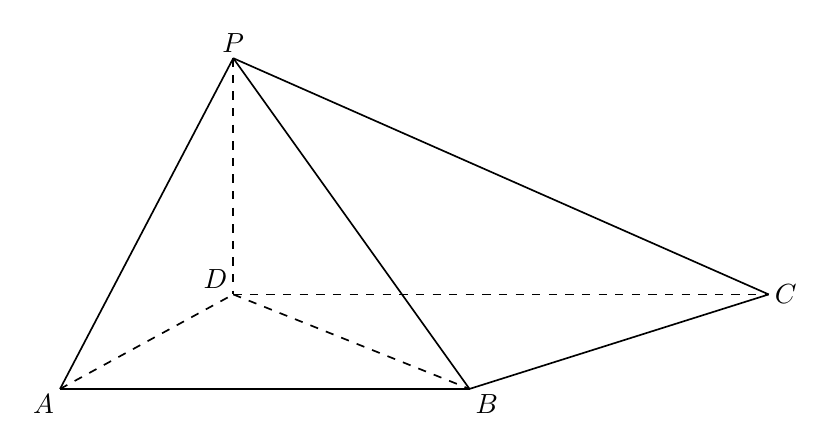
\begin{tikzpicture}[x=1cm,y=1cm,font=\normalsize,
  geometry edge/.style={draw=black,solid,line width=.6pt},
  geometry hidden/.style={draw=black,dashed,line width=.6pt},
  geometry label/.style={font=\normalsize,inner sep=2pt}]
\coordinate (P) at (2.20,4.20);
\coordinate (D) at (2.20,1.20);
\coordinate (A) at (0.00,0.00);
\coordinate (B) at (5.20,0.00);
\coordinate (C) at (9.00,1.20);
\draw[geometry edge] (P)--(A);
\draw[geometry edge] (P)--(B);
\draw[geometry edge] (P)--(C);
\draw[geometry edge] (A)--(B);
\draw[geometry edge] (B)--(C);
\draw[geometry hidden] (P)--(D);
\draw[geometry hidden] (A)--(D);
\draw[geometry hidden] (D)--(B);
\draw[geometry hidden] (D)--(C);
\node[geometry label,above] at (P) {$P$};
\node[geometry label,above left] at (D) {$D$};
\node[geometry label,below left] at (A) {$A$};
\node[geometry label,below right] at (B) {$B$};
\node[geometry label,right] at (C) {$C$};
\end{tikzpicture}
